% Options for packages loaded elsewhere
\PassOptionsToPackage{unicode}{hyperref}
\PassOptionsToPackage{hyphens}{url}
%
\documentclass[
]{article}
\usepackage{lmodern}
\usepackage{amssymb,amsmath}
\usepackage{ifxetex,ifluatex}
\ifnum 0\ifxetex 1\fi\ifluatex 1\fi=0 % if pdftex
  \usepackage[T1]{fontenc}
  \usepackage[utf8]{inputenc}
  \usepackage{textcomp} % provide euro and other symbols
\else % if luatex or xetex
  \usepackage{unicode-math}
  \defaultfontfeatures{Scale=MatchLowercase}
  \defaultfontfeatures[\rmfamily]{Ligatures=TeX,Scale=1}
\fi
% Use upquote if available, for straight quotes in verbatim environments
\IfFileExists{upquote.sty}{\usepackage{upquote}}{}
\IfFileExists{microtype.sty}{% use microtype if available
  \usepackage[]{microtype}
  \UseMicrotypeSet[protrusion]{basicmath} % disable protrusion for tt fonts
}{}
\makeatletter
\@ifundefined{KOMAClassName}{% if non-KOMA class
  \IfFileExists{parskip.sty}{%
    \usepackage{parskip}
  }{% else
    \setlength{\parindent}{0pt}
    \setlength{\parskip}{6pt plus 2pt minus 1pt}}
}{% if KOMA class
  \KOMAoptions{parskip=half}}
\makeatother
\usepackage{xcolor}
\IfFileExists{xurl.sty}{\usepackage{xurl}}{} % add URL line breaks if available
\IfFileExists{bookmark.sty}{\usepackage{bookmark}}{\usepackage{hyperref}}
\hypersetup{
  pdftitle={Lab 1},
  pdfauthor={Emilio Dorigatti},
  hidelinks,
  pdfcreator={LaTeX via pandoc}}
\urlstyle{same} % disable monospaced font for URLs
\usepackage[margin=1in]{geometry}
\usepackage{color}
\usepackage{fancyvrb}
\newcommand{\VerbBar}{|}
\newcommand{\VERB}{\Verb[commandchars=\\\{\}]}
\DefineVerbatimEnvironment{Highlighting}{Verbatim}{commandchars=\\\{\}}
% Add ',fontsize=\small' for more characters per line
\usepackage{framed}
\definecolor{shadecolor}{RGB}{248,248,248}
\newenvironment{Shaded}{\begin{snugshade}}{\end{snugshade}}
\newcommand{\AlertTok}[1]{\textcolor[rgb]{0.94,0.16,0.16}{#1}}
\newcommand{\AnnotationTok}[1]{\textcolor[rgb]{0.56,0.35,0.01}{\textbf{\textit{#1}}}}
\newcommand{\AttributeTok}[1]{\textcolor[rgb]{0.77,0.63,0.00}{#1}}
\newcommand{\BaseNTok}[1]{\textcolor[rgb]{0.00,0.00,0.81}{#1}}
\newcommand{\BuiltInTok}[1]{#1}
\newcommand{\CharTok}[1]{\textcolor[rgb]{0.31,0.60,0.02}{#1}}
\newcommand{\CommentTok}[1]{\textcolor[rgb]{0.56,0.35,0.01}{\textit{#1}}}
\newcommand{\CommentVarTok}[1]{\textcolor[rgb]{0.56,0.35,0.01}{\textbf{\textit{#1}}}}
\newcommand{\ConstantTok}[1]{\textcolor[rgb]{0.00,0.00,0.00}{#1}}
\newcommand{\ControlFlowTok}[1]{\textcolor[rgb]{0.13,0.29,0.53}{\textbf{#1}}}
\newcommand{\DataTypeTok}[1]{\textcolor[rgb]{0.13,0.29,0.53}{#1}}
\newcommand{\DecValTok}[1]{\textcolor[rgb]{0.00,0.00,0.81}{#1}}
\newcommand{\DocumentationTok}[1]{\textcolor[rgb]{0.56,0.35,0.01}{\textbf{\textit{#1}}}}
\newcommand{\ErrorTok}[1]{\textcolor[rgb]{0.64,0.00,0.00}{\textbf{#1}}}
\newcommand{\ExtensionTok}[1]{#1}
\newcommand{\FloatTok}[1]{\textcolor[rgb]{0.00,0.00,0.81}{#1}}
\newcommand{\FunctionTok}[1]{\textcolor[rgb]{0.00,0.00,0.00}{#1}}
\newcommand{\ImportTok}[1]{#1}
\newcommand{\InformationTok}[1]{\textcolor[rgb]{0.56,0.35,0.01}{\textbf{\textit{#1}}}}
\newcommand{\KeywordTok}[1]{\textcolor[rgb]{0.13,0.29,0.53}{\textbf{#1}}}
\newcommand{\NormalTok}[1]{#1}
\newcommand{\OperatorTok}[1]{\textcolor[rgb]{0.81,0.36,0.00}{\textbf{#1}}}
\newcommand{\OtherTok}[1]{\textcolor[rgb]{0.56,0.35,0.01}{#1}}
\newcommand{\PreprocessorTok}[1]{\textcolor[rgb]{0.56,0.35,0.01}{\textit{#1}}}
\newcommand{\RegionMarkerTok}[1]{#1}
\newcommand{\SpecialCharTok}[1]{\textcolor[rgb]{0.00,0.00,0.00}{#1}}
\newcommand{\SpecialStringTok}[1]{\textcolor[rgb]{0.31,0.60,0.02}{#1}}
\newcommand{\StringTok}[1]{\textcolor[rgb]{0.31,0.60,0.02}{#1}}
\newcommand{\VariableTok}[1]{\textcolor[rgb]{0.00,0.00,0.00}{#1}}
\newcommand{\VerbatimStringTok}[1]{\textcolor[rgb]{0.31,0.60,0.02}{#1}}
\newcommand{\WarningTok}[1]{\textcolor[rgb]{0.56,0.35,0.01}{\textbf{\textit{#1}}}}
\usepackage{longtable,booktabs}
% Correct order of tables after \paragraph or \subparagraph
\usepackage{etoolbox}
\makeatletter
\patchcmd\longtable{\par}{\if@noskipsec\mbox{}\fi\par}{}{}
\makeatother
% Allow footnotes in longtable head/foot
\IfFileExists{footnotehyper.sty}{\usepackage{footnotehyper}}{\usepackage{footnote}}
\makesavenoteenv{longtable}
\usepackage{graphicx}
\makeatletter
\def\maxwidth{\ifdim\Gin@nat@width>\linewidth\linewidth\else\Gin@nat@width\fi}
\def\maxheight{\ifdim\Gin@nat@height>\textheight\textheight\else\Gin@nat@height\fi}
\makeatother
% Scale images if necessary, so that they will not overflow the page
% margins by default, and it is still possible to overwrite the defaults
% using explicit options in \includegraphics[width, height, ...]{}
\setkeys{Gin}{width=\maxwidth,height=\maxheight,keepaspectratio}
% Set default figure placement to htbp
\makeatletter
\def\fps@figure{htbp}
\makeatother
\setlength{\emergencystretch}{3em} % prevent overfull lines
\providecommand{\tightlist}{%
  \setlength{\itemsep}{0pt}\setlength{\parskip}{0pt}}
\setcounter{secnumdepth}{-\maxdimen} % remove section numbering
\ifluatex
  \usepackage{selnolig}  % disable illegal ligatures
\fi

\title{Lab 1}
\author{Emilio Dorigatti}
\date{2020-11-06}

\begin{document}
\maketitle

Welcome to the very first lab, in which we will have fun with logistic
regression.

\hypertarget{exercise-1}{%
\subsection{Exercise 1}\label{exercise-1}}

Suppose you have five input points, \(\textbf{x}_1=|0,0|^T\),
\(\textbf{x}_2=|1,0|^T\), \(\textbf{x}_3=|0,-1|^T\),
\(\textbf{x}_4=|-1,0|^T\) and \(\textbf{x}_5=|0,1|^T\), and the
corresponding classes are \(y_1=y_2=y_3=0\) and \(y_4=y_5=1\):

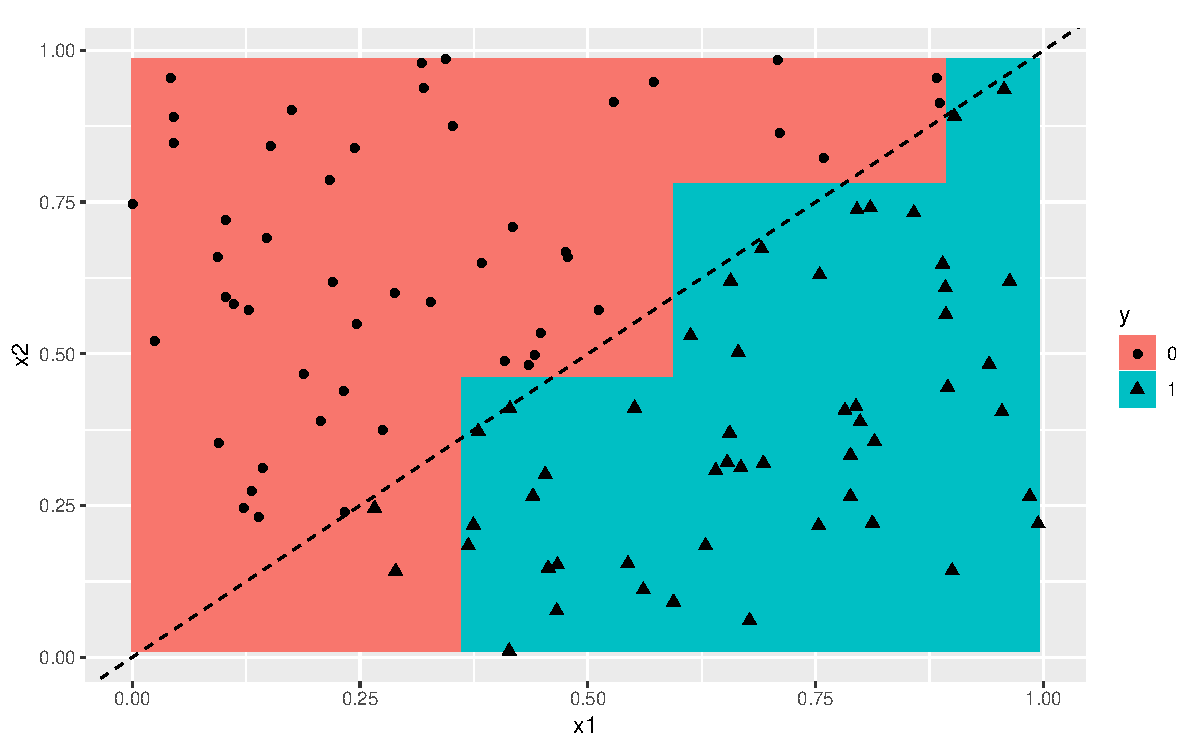
\includegraphics{lab1-questions_files/figure-latex/unnamed-chunk-1-1.pdf}

Consider a logistic regression model
\(\hat{y}_i=\sigma\left(\alpha_0+\alpha_1x_{i1}+\alpha_2x_{i2}\right)\),
with \(\sigma(\cdot)\) the sigmoid function,
\(\sigma(x)=\left(1+e^{-x}\right)^{-1}\). What values for \(\alpha_0\),
\(\alpha_1\) and \(\alpha_2\) would result in the correct classification
for this dataset? A positive label is predicted when the output of the
sigmoid is larger or equal than 0.5.

\begin{center}\rule{0.5\linewidth}{0.5pt}\end{center}

\begin{quote}
\textbf{Note}: do not use any formulas or automated methods to find the
answer. Think for yourself. A logistic regression classifier is nothing
more than a hyper-plane separating points of the two classes. If
necessary, review vectors, dot-products and their geometrical
interpretation in linear algebra. This applies to the following
exercises, too.
\end{quote}

\begin{center}\rule{0.5\linewidth}{0.5pt}\end{center}

\begin{Shaded}
\begin{Highlighting}[]
\NormalTok{a0 }\OtherTok{=}\NormalTok{ (}
  \CommentTok{\# }\AlertTok{TODO}\CommentTok{ fill in the value for alpha 0}
\NormalTok{)}

\NormalTok{a1 }\OtherTok{=}\NormalTok{ (}
  \CommentTok{\# }\AlertTok{TODO}\CommentTok{ fill in the value for alpha 1}
\NormalTok{)}

\NormalTok{a2 }\OtherTok{=}\NormalTok{ (}
  \CommentTok{\# }\AlertTok{TODO}\CommentTok{ fill in the value for alpha 2}
\NormalTok{)}

\CommentTok{\# the first column is always one and is used for the "bias"}
\NormalTok{xs }\OtherTok{=} \FunctionTok{matrix}\NormalTok{(}\FunctionTok{c}\NormalTok{(}
  \DecValTok{1}\NormalTok{, }\DecValTok{0}\NormalTok{, }\DecValTok{0}\NormalTok{,}
  \DecValTok{1}\NormalTok{, }\DecValTok{1}\NormalTok{, }\DecValTok{0}\NormalTok{,}
  \DecValTok{1}\NormalTok{, }\DecValTok{0}\NormalTok{, }\SpecialCharTok{{-}}\DecValTok{1}\NormalTok{,}
  \DecValTok{1}\NormalTok{, }\SpecialCharTok{{-}}\DecValTok{1}\NormalTok{, }\DecValTok{0}\NormalTok{,}
  \DecValTok{1}\NormalTok{, }\DecValTok{0}\NormalTok{, }\DecValTok{1}
\NormalTok{), }\AttributeTok{ncol =} \DecValTok{3}\NormalTok{, }\AttributeTok{byrow =}\NormalTok{ T)}

\NormalTok{sigmoid }\OtherTok{=} \ControlFlowTok{function}\NormalTok{(x) \{}
  \CommentTok{\# }\AlertTok{TODO}\CommentTok{ compute and return the sigmoid transformation on x}
\NormalTok{\}}

\FunctionTok{sigmoid}\NormalTok{(xs }\SpecialCharTok{\%*\%} \FunctionTok{c}\NormalTok{(a0, a1, a2))}
\end{Highlighting}
\end{Shaded}

You should make sure that the last two values are close to one, and the
others are close to zero.

\hypertarget{exercise-2}{%
\subsection{Exercise 2}\label{exercise-2}}

Continuing from the previous exercise, suppose now that \(y_2=y_3=1\)
and \(y_1=y_2=y_5=0\):

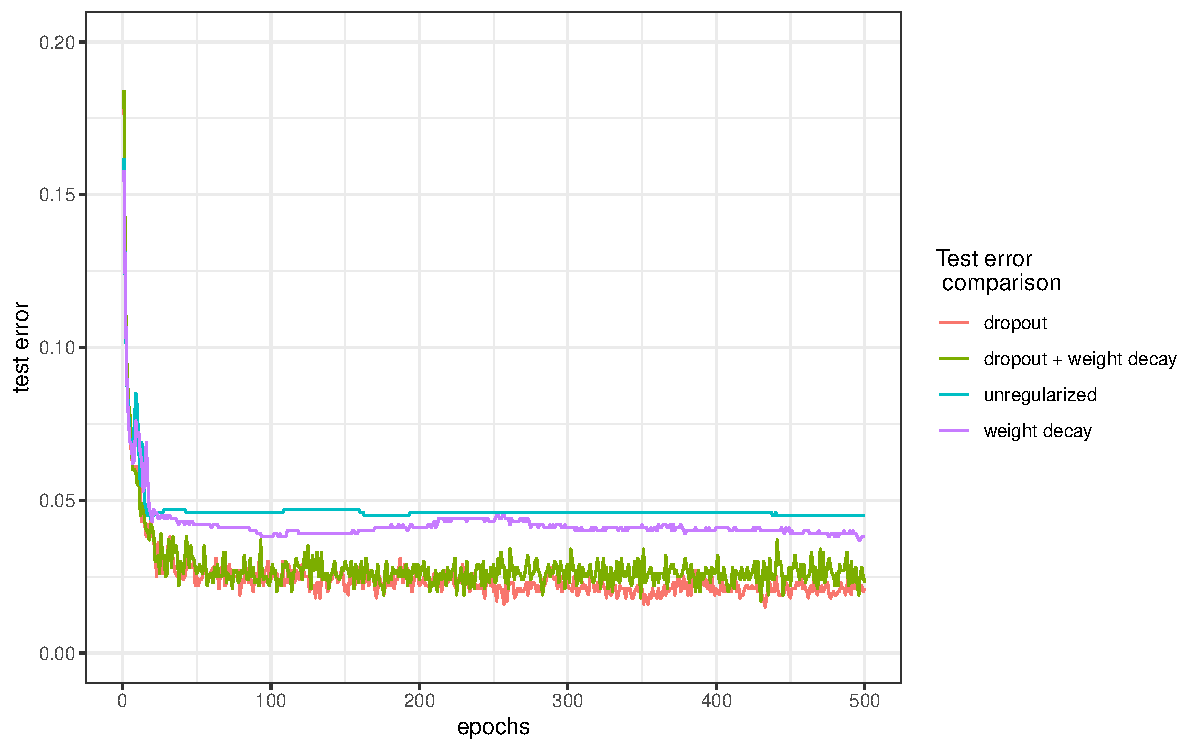
\includegraphics{lab1-questions_files/figure-latex/unnamed-chunk-3-1.pdf}

Consider the same logistic regression model above with coefficients
\(\beta_0\), \(\beta_1\) and \(\beta_2\), how would you need to set
these coefficients to correctly classify this dataset?

\begin{Shaded}
\begin{Highlighting}[]
\NormalTok{b0 }\OtherTok{=}\NormalTok{ (}
  \CommentTok{\# }\AlertTok{TODO}\CommentTok{ fill in the value for beta 0}
\NormalTok{)}

\NormalTok{b1 }\OtherTok{=}\NormalTok{ (}
  \CommentTok{\# }\AlertTok{TODO}\CommentTok{ fill in the value for beta 1}
\NormalTok{)}

\NormalTok{b2 }\OtherTok{=}\NormalTok{ (}
  \CommentTok{\# }\AlertTok{TODO}\CommentTok{ fill in the value for beta 2}
\NormalTok{)}

\FunctionTok{sigmoid}\NormalTok{(xs }\SpecialCharTok{\%*\%} \FunctionTok{c}\NormalTok{(b0, b1, b2))}
\end{Highlighting}
\end{Shaded}

Make sure that the second and third elements are close to one, and the
others close to zero.

\hypertarget{exercise-3}{%
\subsection{Exercise 3}\label{exercise-3}}

Finally, with the same data as before, suppose that \(y_1=1\) and
\(y_2=y_3=y_4=y_5=0\):

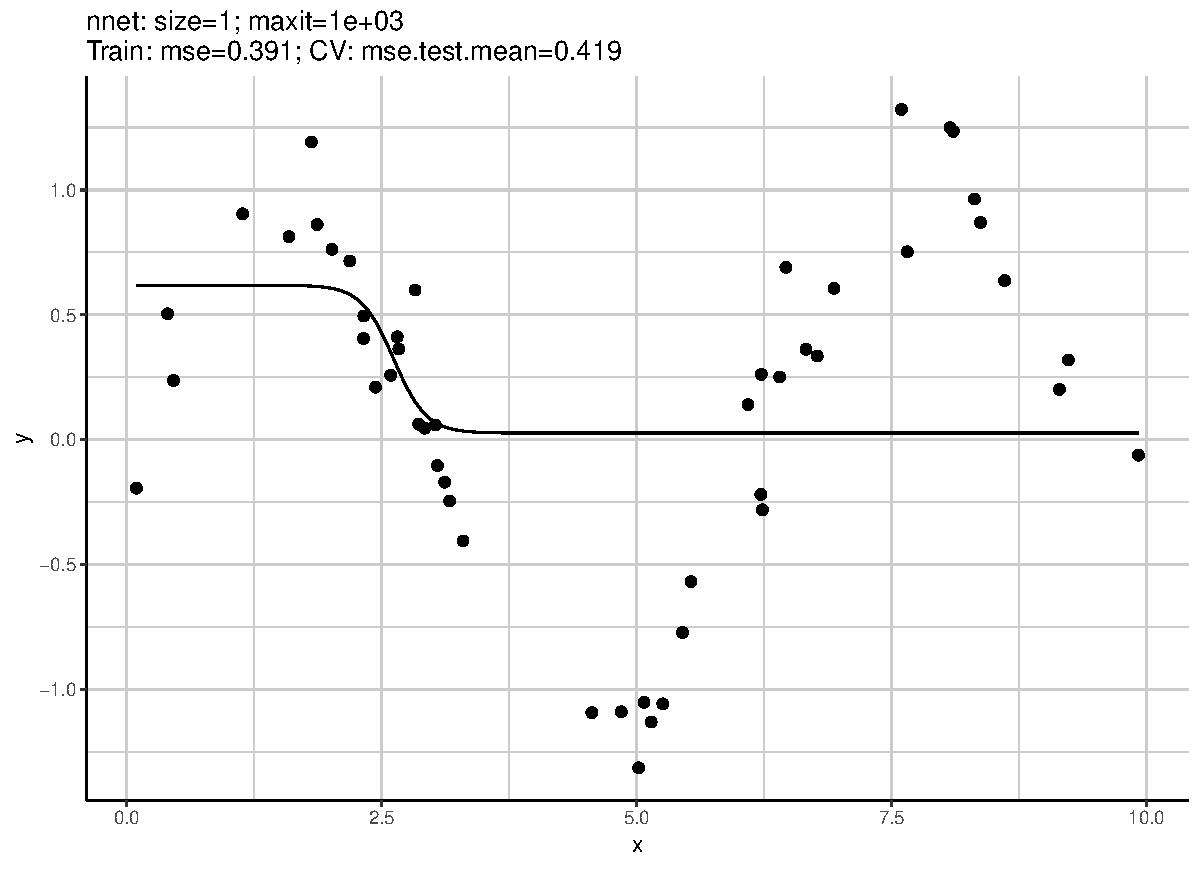
\includegraphics{lab1-questions_files/figure-latex/unnamed-chunk-5-1.pdf}

Clearly, logistic regression cannot correctly classify this dataset,
since the two classes are not linearly separable (optional: prove it,
see solution at the bottom).

However, as we have shown in the previous exercises, it is possible to
separate \(x_2\) and \(x_3\) from the rest, and \(x_4\) and \(x_5\) from
the rest.

Can these two simple classifiers be composed into one that is powerful
enough to separate \(x_1\) from the rest?

Can we use their predictions as input for another logistic regression
classifier?

Let \(z_{i1}=\sigma(\alpha_0+\alpha_1x_{i1}+\alpha_2x_{i2})\) and
\(z_{i2}=\sigma(\beta_0+\beta_1x_{i1}+\beta_2x_{i2})\) be the output of
the two logistic regression classifiers for point \(i\). Then, the
dataset would become:

\begin{longtable}[]{@{}llll@{}}
\toprule
\(i\) & \(z_{i1}\) & \(z_{i2}\) & \(y\)\tabularnewline
\midrule
\endhead
\(1\) & 0 & 0 & 1\tabularnewline
\(2\) & 0 & 1 & 0\tabularnewline
\(3\) & 0 & 1 & 0\tabularnewline
\(4\) & 1 & 0 & 0\tabularnewline
\(5\) & 1 & 0 & 0\tabularnewline
\bottomrule
\end{longtable}

In graphical form:

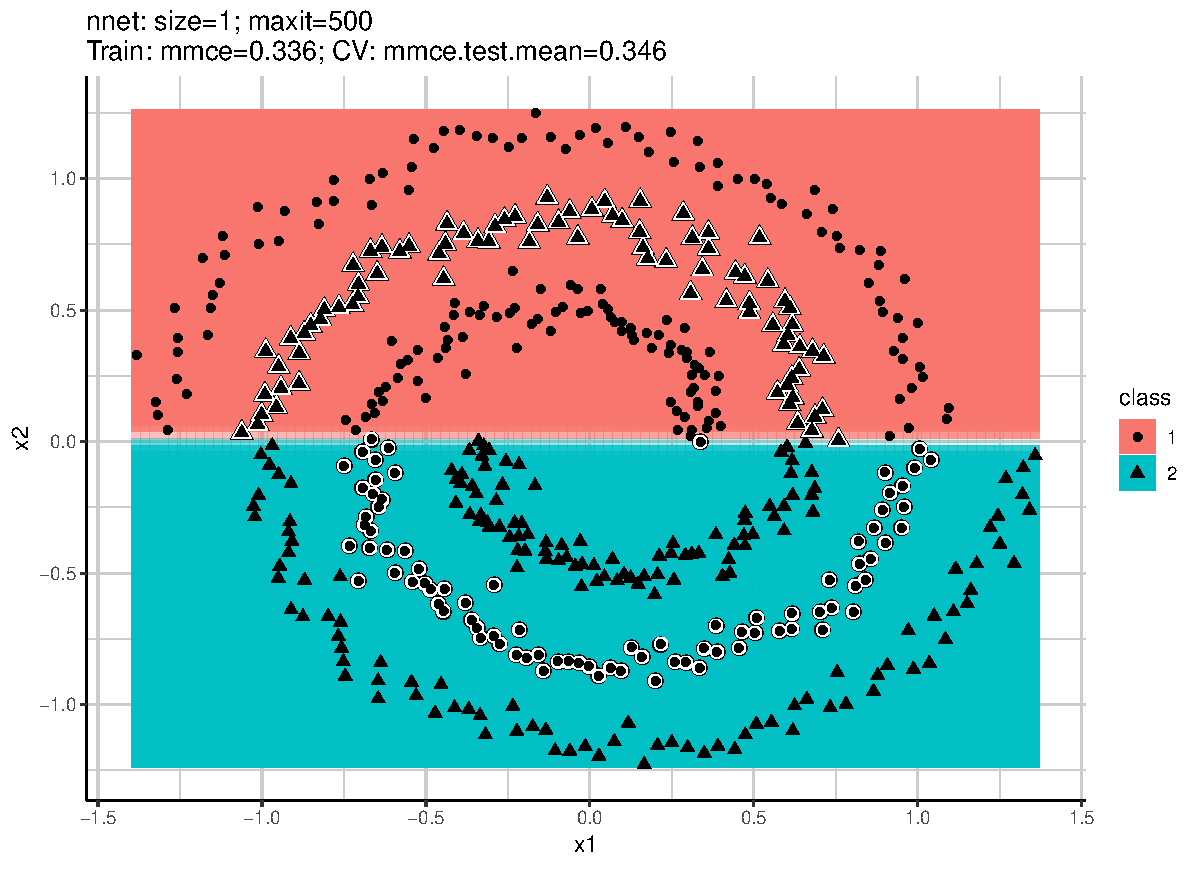
\includegraphics{lab1-questions_files/figure-latex/unnamed-chunk-6-1.pdf}

This sure looks linearly separable! As before, find the coefficients for
a linear classifier
\(\hat{y}_i=\sigma\left(\gamma_0+\gamma_1z_{i1}+\gamma_2z_{i2}\right)\):

\begin{Shaded}
\begin{Highlighting}[]
\NormalTok{g0 }\OtherTok{=}\NormalTok{ (}
  \CommentTok{\# }\AlertTok{TODO}\CommentTok{ fill in the value for gamma 0}
\NormalTok{)}

\NormalTok{g1 }\OtherTok{=}\NormalTok{ (}
  \CommentTok{\# }\AlertTok{TODO}\CommentTok{ fill in the value for gamma 1}
\NormalTok{)}

\NormalTok{g2 }\OtherTok{=}\NormalTok{ (}
  \CommentTok{\# }\AlertTok{TODO}\CommentTok{ fill in the value for gamma 2}
\NormalTok{)}

\NormalTok{zs }\OtherTok{=} \FunctionTok{matrix}\NormalTok{(}\FunctionTok{c}\NormalTok{(}
  \DecValTok{1}\NormalTok{, }\DecValTok{0}\NormalTok{, }\DecValTok{0}\NormalTok{,}
  \DecValTok{1}\NormalTok{, }\DecValTok{0}\NormalTok{, }\DecValTok{1}\NormalTok{,}
  \DecValTok{1}\NormalTok{, }\DecValTok{0}\NormalTok{, }\DecValTok{1}\NormalTok{,}
  \DecValTok{1}\NormalTok{, }\DecValTok{1}\NormalTok{, }\DecValTok{0}\NormalTok{,}
  \DecValTok{1}\NormalTok{, }\DecValTok{1}\NormalTok{, }\DecValTok{0}
\NormalTok{), }\AttributeTok{ncol =} \DecValTok{3}\NormalTok{, }\AttributeTok{byrow =}\NormalTok{ T)}

\FunctionTok{sigmoid}\NormalTok{(zs }\SpecialCharTok{\%*\%} \FunctionTok{c}\NormalTok{(g0, g1, g2))}
\end{Highlighting}
\end{Shaded}

Make sure that the first element is close to one, and the others close
to zero.

This big classifier can be summarized as follows:

\begin{Shaded}
\begin{Highlighting}[]
\NormalTok{z1 }\OtherTok{=} \FunctionTok{sigmoid}\NormalTok{(xs }\SpecialCharTok{\%*\%} \FunctionTok{c}\NormalTok{(a0, a1, a2))}
\NormalTok{z2 }\OtherTok{=} \FunctionTok{sigmoid}\NormalTok{(xs }\SpecialCharTok{\%*\%} \FunctionTok{c}\NormalTok{(b0, b1, b2))}

\NormalTok{yhat }\OtherTok{=} \FunctionTok{sigmoid}\NormalTok{(g0 }\SpecialCharTok{+}\NormalTok{ g1 }\SpecialCharTok{*}\NormalTok{ z1 }\SpecialCharTok{+}\NormalTok{ g2 }\SpecialCharTok{*}\NormalTok{ z2)}
\NormalTok{yhat}
\end{Highlighting}
\end{Shaded}

And this is just what a neural network looks like! Each neuron is a
simple linear classifier, and we just stack linear classifiers on top of
linear classifiers. And we could go on and on, with many layers of
linear classifiers.

\hypertarget{proof-sketch-that-this-dataset-is-not-linearly-separable}{%
\subsubsection{Proof sketch that this dataset is not linearly
separable}\label{proof-sketch-that-this-dataset-is-not-linearly-separable}}

The \emph{convex hull} of a set of points is the smallest convex polygon
that encloses them. In our case, the convex hull of \(x_2,\ldots,x_5\)
is a square with those points as vertices.

\end{document}
